\documentclass{../source/zjureport}

\major{信息工程}
\name{周灿松}
\title{实验设计报告}
\stuid{3190105055}
\college{信息与电子工程学院}
\date{\today}
\lab{教4-421}
\course{数字信号处理}
\instructor{徐元欣}
\grades{}
\expname{FIR数字滤波器设计与使用}
\exptype{综合}
\partner{--}

\begin{document}
    \makeheader

    \section{实验目的和要求}
    设计和应用FIR低通滤波器。掌握FIR数字滤波器的窗函数设计法,了解设计参数(窗型、窗长)的影响。

    \section{实验内容和步骤}
    编写MATLAB程序,完成以下工作。
        \subsection{设计两个FIR低通滤波器,截止频率$\omega_c = 0.5\pi$}
            \begin{enumerate}
                \item 用矩形窗,窗长$N=31$。得出第一个滤波器的单位抽样响应序列$h_1(n)$。记下$h_1(n)$的各个抽样值,显示$h_1(n)$的图形(用stem(.))。求出该滤波器的频率响应(的N个抽样)$H_1(k)$,显示$|H_1(k)|$的图形(用plot(.))。
                \item 用汉明窗,窗长N=31。得出第二个滤波器的单位抽样响应序列$h_2(n)$。记下$h_2(n)$的各个抽样值,显示$h_2(n)$的图形。求出滤波器的频率响应$H_2(k)$,显示$|H_2(k)|$的图形。
                \item 由图形,比较$h_1(n)$与$h_2(n)$的差异,$|H_1(k)|$与$|H_2(k)|$的差异。
            \end{enumerate}
        \subsection{产生长度为200点、均值为零的随机信号序列x(n)(用rand(1,200)-0.5)。显示x(n)。求出并显示其幅度谱|X(k)|,观察特征。}
        \subsection{滤波}
            \begin{enumerate}
                \item 将$x(n)$作为输入,经过第一个滤波器后的输出序列记为$y_1(n)$,其幅度谱记为$|Y_1(k)|$。显示$|X(k)|$与$|Y_1(k)|$,讨论滤波前后信号的频谱特征。
                \item 将$x(n)$作为输入,经过第二个滤波器后的输出序列记为$y_2(n)$,其幅度谱记为$|Y_2(k)|$。比较$|Y_1(k)|$与$|Y_2(k)|$的图形,讨论不同的窗函数设计出的滤波器的滤波效果。
            \end{enumerate}
        \subsection{设计第三个FIR低通滤波器,截止频率$\omega_c = 0.5\pi$。用矩形窗,窗长$N=127$。用它对$x(n)$进行滤波。显示输出信号$y_3(n)$的幅度谱$|Y_3(k)|$,并与$|Y_1(k)|$比较,讨论不同的窗长设计出的滤波器的滤波效果。}
    
    \section{主要仪器设备}
    自行编程。

    \section{操作方法和实验步骤}
    (参见“二、实验内容和步骤”)

    \section{实验数据记录和处理}
        \subsection{MATLAB代码}
            \lstinputlisting[caption = 实验代码 , language = matlab]{code/Lab4.m}

        \subsection{计算结果}
            \begin{figure}[H]
                \centering
                \begin{minipage}[t]{0.48\textwidth}
                \centering
                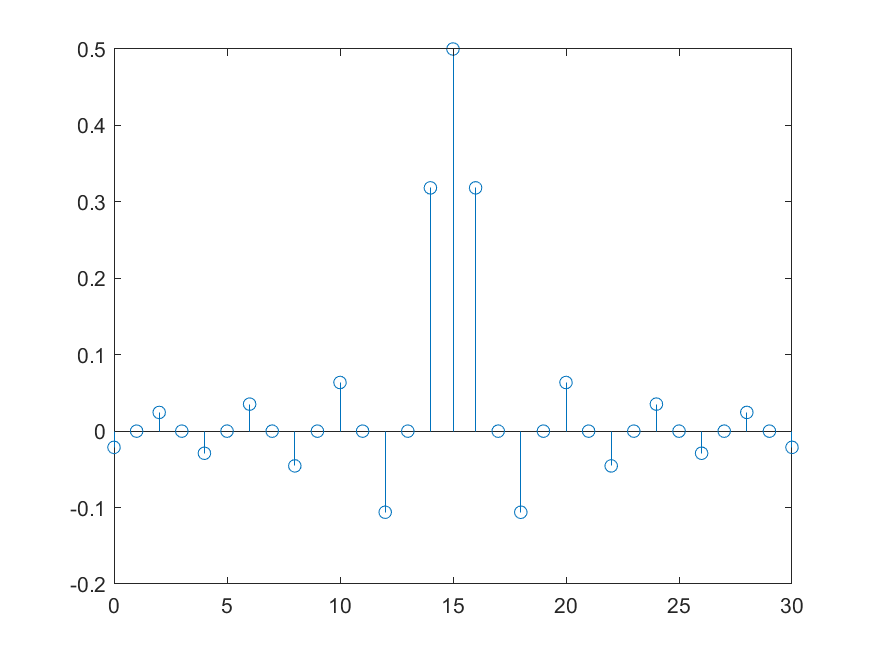
\includegraphics[width=\textwidth]{figure/h1.png}
                \caption{$h_1(n)$}
                \end{minipage}
                \begin{minipage}[t]{0.48\textwidth}
                \centering
                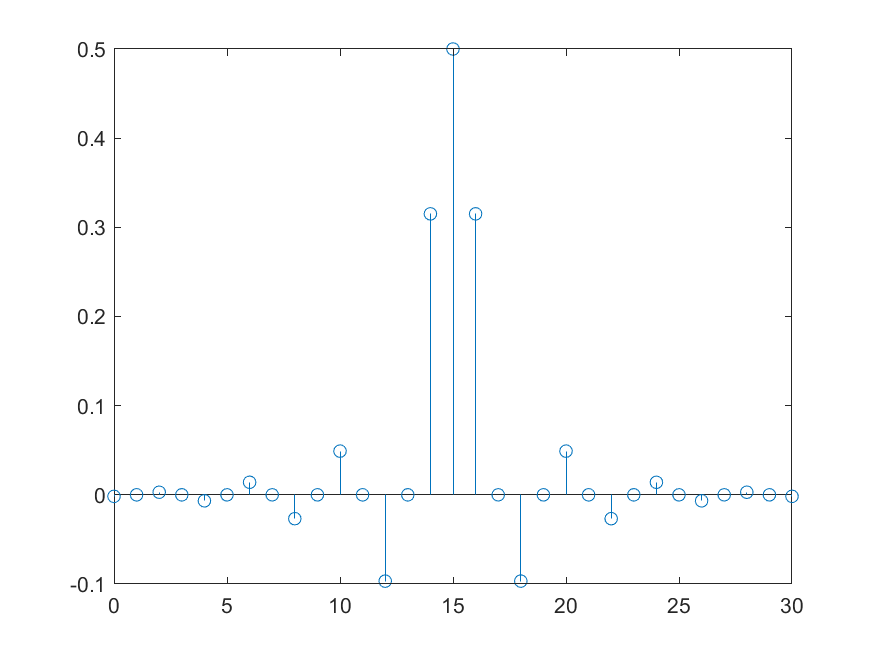
\includegraphics[width=\textwidth]{figure/h2.png}
                \caption{$h_2(n)$}
                \end{minipage}
            \end{figure}

            
            \begin{figure}[H]
                \centering
                \begin{minipage}[H]{0.32\textwidth}
                    \centering
                    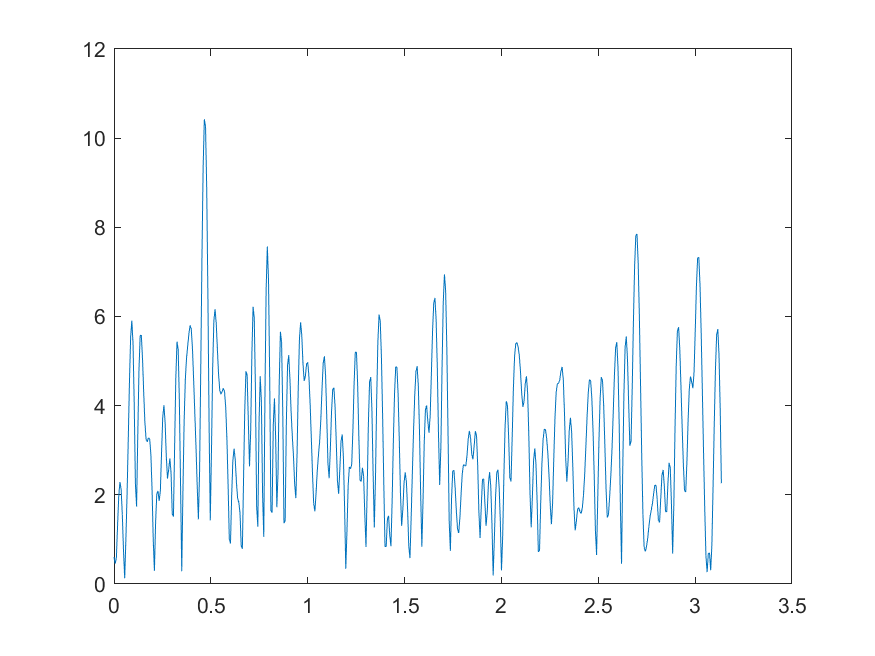
\includegraphics[width=\textwidth]{figure/X(k).png}
                    \caption{$|X(k)|$}
                \end{minipage}
                \begin{minipage}[H]{0.32\textwidth}
                    \centering
                    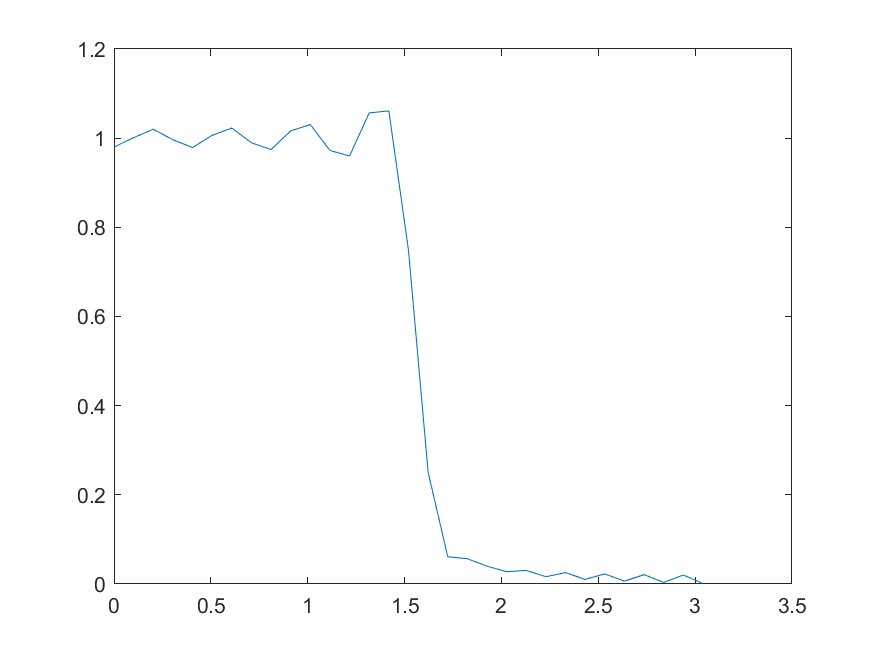
\includegraphics[width=\textwidth]{figure/H_1.png}
                    \caption{$|H_1(k)|$}
                \end{minipage}
                \begin{minipage}[H]{0.32\textwidth}
                    \centering
                    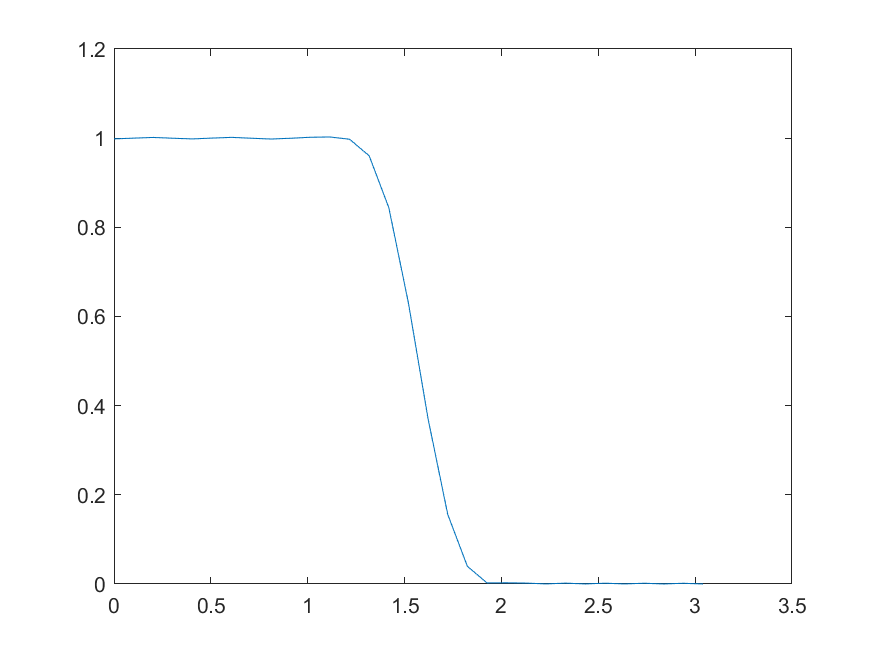
\includegraphics[width=\textwidth]{figure/H_2.png}
                    \caption{$|H_2(k)|$}
                \end{minipage}
            \end{figure}

            \begin{figure}[H]
                \centering
                \begin{minipage}[H]{0.32\textwidth}
                    \centering
                    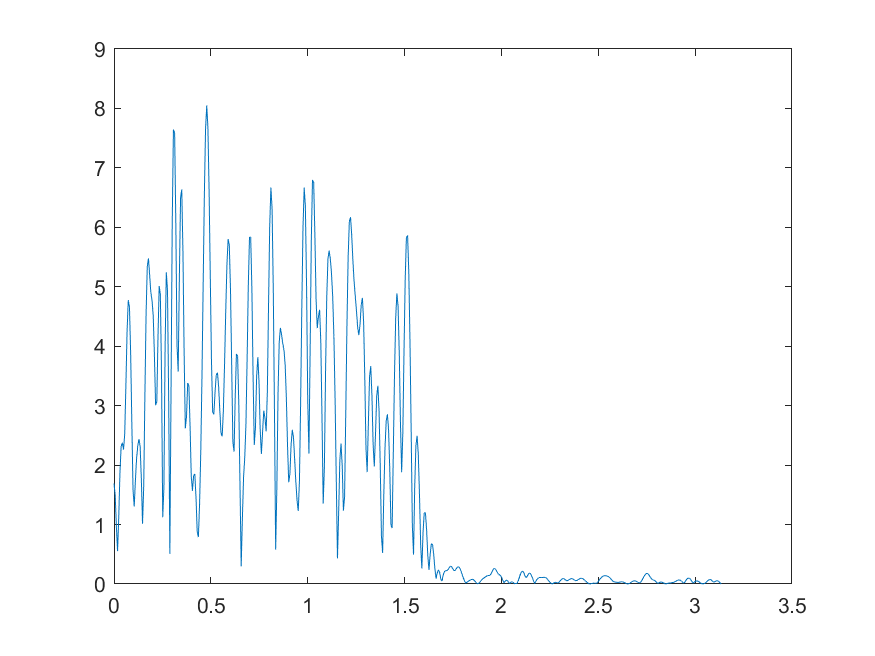
\includegraphics[width=\textwidth]{figure/Y1(k).png}
                    \caption{$|Y_1(k)|$}
                \end{minipage}
                \begin{minipage}[H]{0.32\textwidth}
                    \centering
                    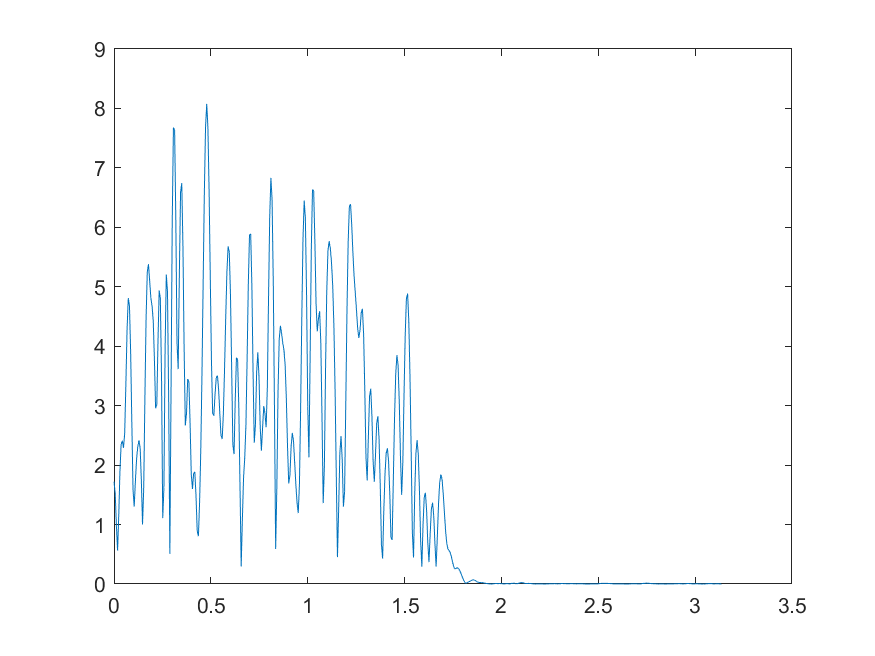
\includegraphics[width=\textwidth]{figure/Y2(k).png}
                    \caption{$|Y_2(k)|$}
                \end{minipage}
                \begin{minipage}[H]{0.32\textwidth}
                    \centering
                    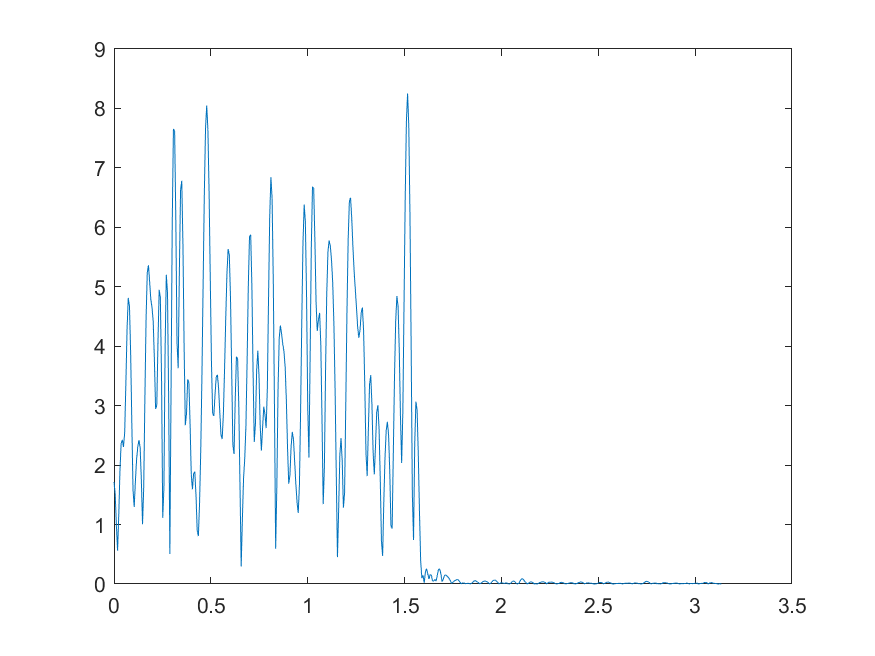
\includegraphics[width=\textwidth]{figure/Y3(k).png}
                    \caption{$|Y_3(k)|$}
                \end{minipage}
            \end{figure}

    \section{实验结果与分析}
        \subsection{$h_1(n)$与$h_2(n)$的差异}
            \begin{figure}[H]
                \centering
                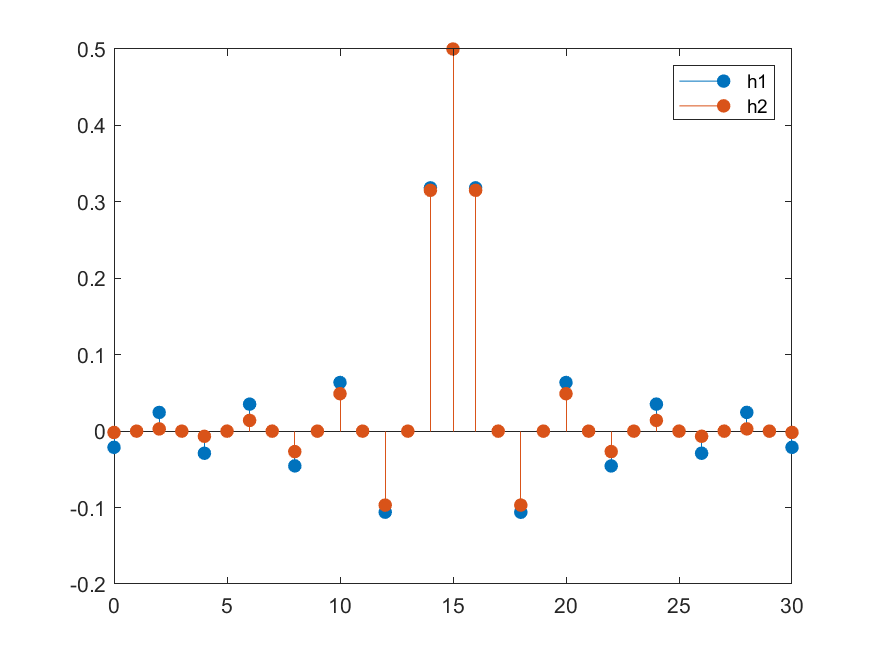
\includegraphics[scale = 0.7]{figure/h区别.png}
                \caption{$h_1(n)$与$h_2(n)$的差异}
            \end{figure}
        观察图像可以看出:$h_2(n)$远离中心的点的幅度比$h_1(n)$要低

        \subsection{$X(k)的频率特性$}
        有$x(n)$的幅度谱可以看出,其幅度在所有频段均匀分布

        \subsection{$|H_1(k)|$与$|H_2(k)|$的差异}
        \begin{figure}[H]
            \centering
            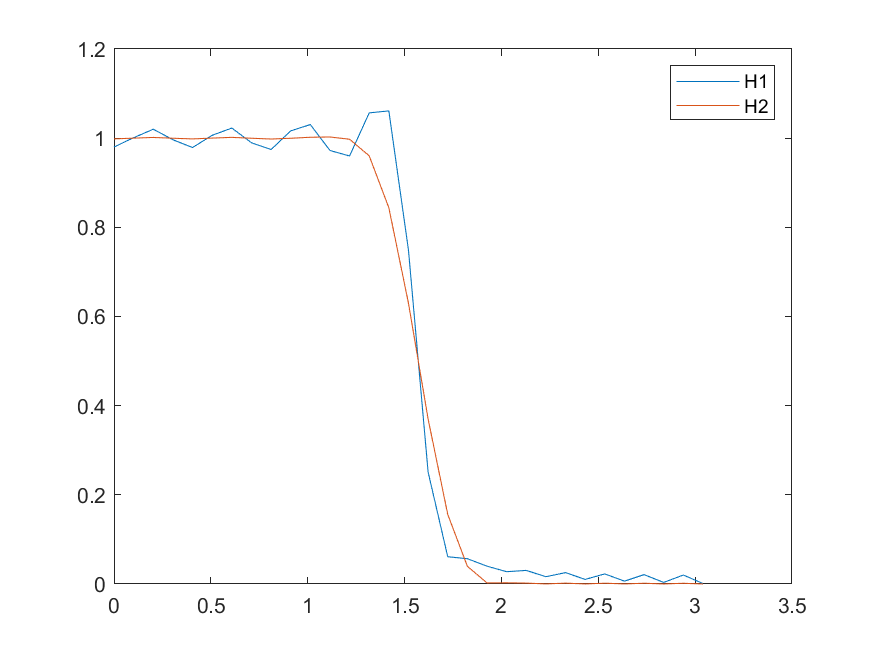
\includegraphics[scale = 0.7]{figure/频响区别.png}
            \caption{$|H_1(k)|$与$|H_2(k)|$的差异}
        \end{figure}
        由图像可以看出:$|H_1(k)|$在通带和阻带中有波动,而$|H_2(k)|$没有;但是$|H_1(k)|$有着更加陡峭的过渡带。



        \subsection{滤波前后信号的频谱特征}
        \begin{figure}[H]
            \centering
            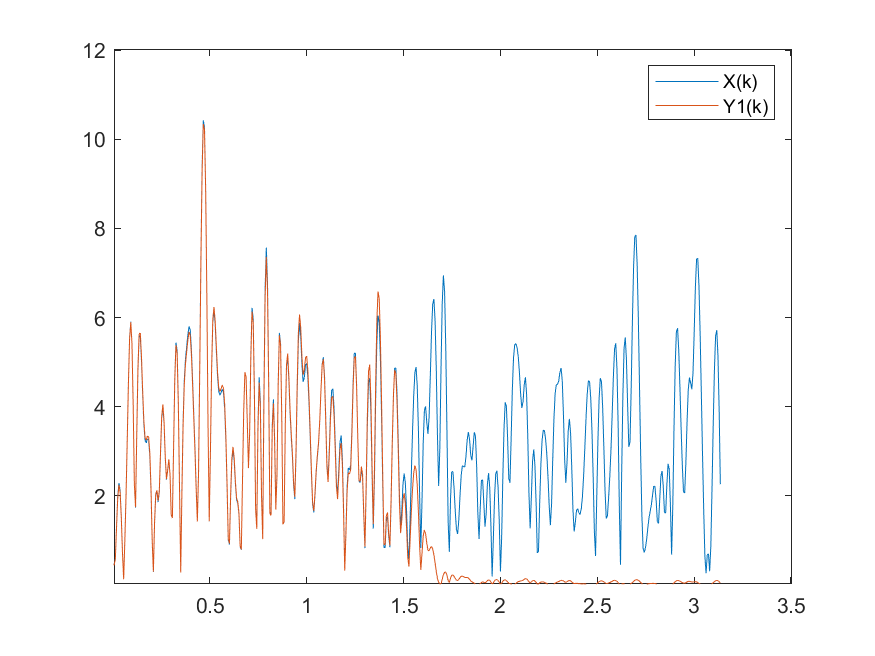
\includegraphics[scale = 0.7]{figure/X(k)与Y1(k)区别.png}
            \caption{滤波前后信号的频谱特征}
        \end{figure}
        如图可得:在滤波之后,$X(k)$的低于截止频率的部分依旧保留,高于截至频率的部分被滤波器滤除。

        \subsection{不同的窗函数设计出的滤波器的滤波效果}
        \begin{figure}[H]
            \centering
            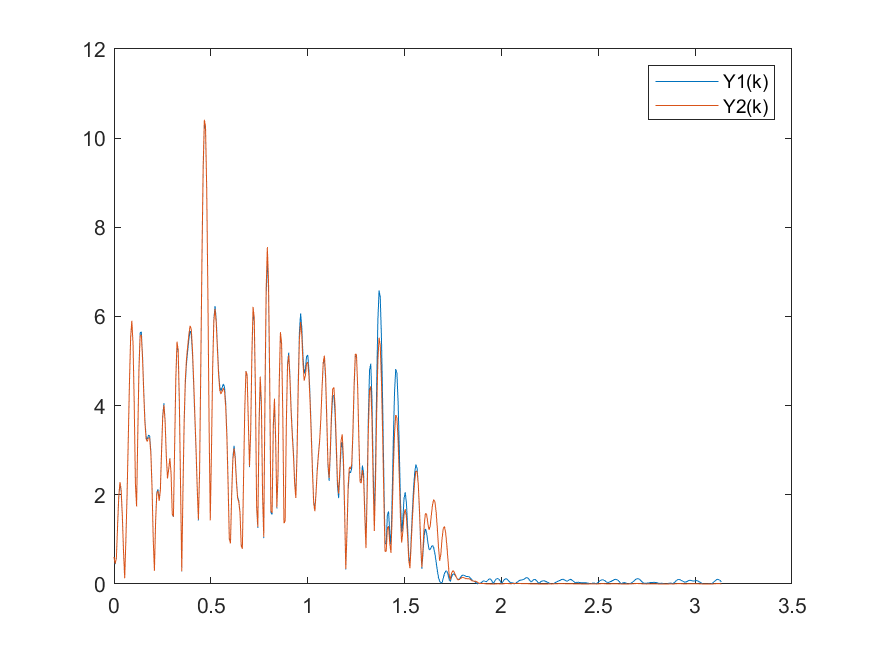
\includegraphics[scale = 0.7]{figure/Y2(k)与Y1(k)区别.png}
            \caption{不同的窗函数设计出的滤波器的滤波效果}
        \end{figure}
        由图可知:当窗函数长度相等时,使用矩形窗能够获得更陡峭的过渡带,但是最小阻带衰减比汉明窗更大

        \subsection{不同的窗长设计出的滤波器的滤波效果}
        \begin{figure}[H]
            \centering
            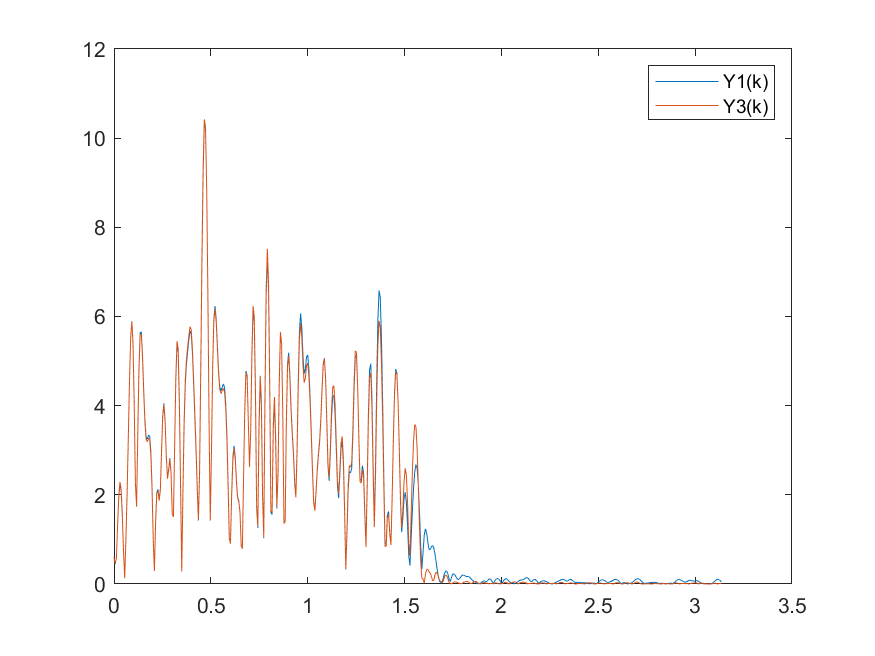
\includegraphics[scale = 0.6]{figure/Y3(k)与Y1(k)区别.png}
            \caption{不同的窗长设计出的滤波器的滤波效果}
        \end{figure}
        由图可知:当窗的长度增加时,滤波器的过渡带变得更加得陡峭,阻带内的绝对振幅减弱。

        \subsection{总结}
        滤波器的频率响应的过渡带宽主要取决于选用的窗函数的种类以及窗长,不同的窗函数有着过渡带宽不同同时当窗长增加时,过渡带会变窄。

        阻带最小衰减主要取决于窗函数的种类,矩形窗、三角窗、汉宁窗、汉明窗、布莱克曼窗的最小阻带衰减依次减小

\end{document}